\documentclass[12pt, a4paper]{article}
\usepackage{hyperref}
\usepackage{graphicx}
	\graphicspath{{figures/}}
\usepackage[bottom]{footmisc}
\usepackage{setspace}
\usepackage[font=footnotesize]{caption}
\usepackage{graphicx,caption}
\usepackage[super,comma]{natbib}
\renewcommand{\thefootnote}{\alph{footnote}}

\title{
    \vspace{-25mm}
    \large \bfseries Streamlined and Interactive Analysis and Pathway-Mapping of Targeted Metabolomics Data from the Biocrates Platform Using MetAlyzer
    \vspace{-4mm}
    }
\author{
    \vspace{-2mm}
    \hspace{-124mm} \small \textbf{Author list:}\\
    \vspace{-3mm} \small Qian-Wu Liao*, Luis Herfurth*, Christina Schmidt*, Nils Mechtel, Hagen M. Gegner,\\
    \hspace{-41mm} \small Alice Limonciel, Rüdiger Hell, Junyan Lu and Gernot Poschet\\
    \hspace{-37mm} \vspace{-3mm} \small \textbf{Corresponding:} Junyan Lu (junyan.lu@uni-heidelberg.de) and\\
    \hspace{9mm} \small Gernot Poschet (gernot.poschet@cos.uni-heidelberg.de)
    }
\date{}

\setstretch{1.5}

\begin{document}
\maketitle

\section*{\large Abstract}
Mass spectrometry (MS)-based metabolomics has emerged as a powerful tool to address multifaceted biological questions. Biocrates, a biotechnology company, has developed standardized, ready-to-use kits for reliable metabolic profiling. Raw MS data from these kits are typically quantified and preprocessed using Biocrates' WebIDQ software, which exports an Excel spreadsheet containing metabolite concentrations along with sample and metabolite metadata. However, the output spreadsheet is complex; for example, the quality status of each measurement is by default color-coded, making downstream bioinformatic analysis and data exploration challenging. To address this, we developed MetAlyzer, an R package specifically designed to handle Biocrates-exported data. MetAlyzer converts complex spreadsheets into flexible \textit{SummarizedExperiment} objects and provides functions for data preprocessing, statistical testing, and visualization of differential metabolites. To further support data exploration and hypothesis generation by users without coding experience, we also developed an interactive and intuitive Shiny app that interfaces with MetAlyzer's core functionality, enabling users to execute the complete analysis workflow without writing code. This combination can help advance metabolomics research in the life sciences.

\section*{\large Introduction}
Metabolomics aided by mass spectrometry (MS) technologies has become a powerful tool for investigating intricate biochemical networks within living organisms and is applied across diverse fields such as biomedical, nutritional, and agricultural sciences\cite{Gowda2008,Gomez-Casati2013,Gonzalez-Covarrubias2022}. While global metabolic profiling has attracted significant interest over the past decades due to its comprehensive coverage and discovery potential, targeted metabolomics offers unique advantages in specificity, sensitivity, and reproducibility by focusing on the precise measurement and quantification of predefined sets of metabolites\cite{Begou2017}.

To achieve reliable MS-based metabolomics analysis, Biocrates, a biotechnology company, has designed ready-to-use kits that provide quantitative, standardized, and reproducible assays covering more than 1,000 metabolites across over 40 metabolite classes (Biocrates, Austria). Raw MS data from these kits are typically quantified and preprocessed by Biocrates' WebIDQ, a proprietary software that transforms MS raw intensities into precise metabolite concentrations and outputs an informative but complex Excel spreadsheet. In addition to concentrations, the output includes color-coded quantification statuses along with sample and metabolite metadata, whose complexity presents challenges for downstream statistical analysis and interpretability. Therefore, a user-friendly tool that can convert this information-rich but unstructured data into a common data structure (e.g., a data frame) is urgently needed to enable better use of Biocrates data by bioinformaticians and wet-lab biologists.

Several web-based platforms can process and analyze targeted metabolomics data, such as MetaboAnalyst\cite{Pang2024}, Galaxy\cite{Galaxy2024}, and Metabolomics Workbench\cite{MWB}. However, none of these tools can be directly applied to spreadsheets exported from WebIDQ. MeTaQuaC\cite{Kuhring2020}, a published R package, was developed to perform automated quality control of targeted metabolomics data, particularly from the Biocrates platform, and produces reports in HTML format. However, MeTaQuaC and its static reports lack the flexibility for customized data processing and analysis required to answer specific biological questions.

To overcome these limitations, we developed \textbf{MetAlyzer}, which aims to facilitate the parsing of WebIDQ outputs, enable flexible analysis, and improve the accessibility of targeted metabolomics data from the Biocrates platform. With a dual-mode design that combines a code-based R interface and an interactive Shiny interface within a single package, MetAlyzer accommodates both experienced bioinformaticians and wet-lab biologists with limited coding experience. In conjunction with the Biocrates platform, we envision MetAlyzer as a complementary and powerful tool for advancing accessible and reproducible metabolomics research in the life sciences. We demonstrate the usability and functionality of MetAlyzer using a demo dataset generated with the MxP® Quant 500 XL kit, provided by our collaborators at Biocrates, in the Results section.

% MetAlyzer offers a streamlined workflow for processing, analysis, and visualization of targeted metabolomics datasets acquired through the biocrates platform. A core initial function of MetAlyzer is converting a complex Excel spreadsheet exported from biocrates' \textbf{MetIDQ} software into a flexible, widely-used \textit{SummarizedExperiment} object\cite{Morgan2022} that keeps the original information. This conversion enhances data accessibility and interoperability, enabling users to use tools provided by both MetAlyzer and external resources such as the Bioconductor ecosystem\cite{Huber2015}. As a one-stop solution for data processing and analysis, MetAlyzer supports sample and metabolite filtering, data imputation and transformation, quality control, statistical analysis, and visualization of differential metabolites. One standout feature of MetAlyzer is its contextual visualization of metabolite-level statistics mapped onto canonical metabolic pathways, which facilitates the identification of biologically relevant metabolites and their interconnections. Moreover, recognizing that coding can be intimidating for users with limited programming experience, we also developed an interactive Shiny app that interfaces with MetAlyzer's core functionality and provides point-and-click access to the full analysis workflow without requiring any coding. Several web-based platforms for metabolomics data processing and analysis exist, such as MetaboAnalyst\cite{Pang2024}, Galaxy\cite{Galaxy2024}, and Metabolomics Workbench\cite{MWB}. However, none of these tools can be directly applied to spreadsheets exported from the \textbf{MetIDQ} software. For instance, if users wish to perform statistical analysis using MetaboAnalyst, they must first convert the output spreadsheet into a concentration matrix. Although MetaboAnalyst provides a comprehensive set of preprocessing options throughout its analysis workflow, users may find it difficult to select appropriate operations without an initial overview of the dataset. In contrast, Shiny-based MetAlyzer can directly handle biocrates-exported datasets and provides immediate visual feedback for each operation. Collectively, the aforementioned features establish MetAlyzer as an efficient, flexible, and reproducible solution that bridges the gap between raw biocrates output and custom downstream analysis.

\section*{\large Results}
\subsection*{\normalsize Overall features}
MetAlyzer provides a workflow for processing, quality control, statistical analysis, and visualization of targeted metabolomics datasets generated using the Biocrates platform. The workflow begins by converting an Excel spreadsheet (.xlsx format; Fig.~\ref{fig:overallFeatures}A) exported from the WebIDQ software into a \textit{SummarizedExperiment} object\cite{Morgan2022}, which serves as the central data structure for subsequent preprocessing and downstream analysis. MetAlyzer supports sample and metabolite filtering, half-minimum imputation, $\log_2$ transformation, and various analyses including descriptive statistics, fold changes (FCs), and ANOVA. Visual summaries of differential metabolites are generated as volcano plots, scatter plots, and metabolic network diagrams (Fig.~\ref{fig:overallFeatures}B). In addition to the R-based interface, MetAlyzer includes a Shiny-based graphical interface\cite{Chang2024} that offers point-and-click access to its core functionality (Fig.~\ref{fig:overallFeatures}C). The app delivers real-time visual feedback for each preprocessing operation, including boxplots of metabolite concentration distributions across samples and barplots of metabolite missing values and quantification statuses. All preprocessing parameters and their corresponding outputs are logged in a history table, enabling traceability and comparisons of different configurations. For statistical analysis, volcano plots allow users to adjust $\log_2$ FC and p-value cutoffs and highlight specific metabolites or metabolic classes; scatter plots show associations between $\log_2$ FCs and metabolic classes.

Another standout feature of MetAlyzer is its contextual visualization of metabolite-level statistics through network diagrams. These diagrams map $\log_2$ FCs and p-values directly onto curated canonical metabolic pathways, such as the TCA cycle, $\beta$-oxidation, and glutamate metabolism, which facilitates the identification of biologically relevant metabolites and their interconnections. All visualizations supported by the app are interactive and can be exported in HTML, PDF, SVG, or PNG formats.
% Additionally, users can retrieve alternative metabolite identifiers (e.g., HMDB IDs) corresponding to Biocrates-named compounds for downstream applications outside MetAlyzer.

\begin{figure}[h!]
    \centering
    \captionsetup{width=1.02\linewidth}
    \hspace{-6mm} 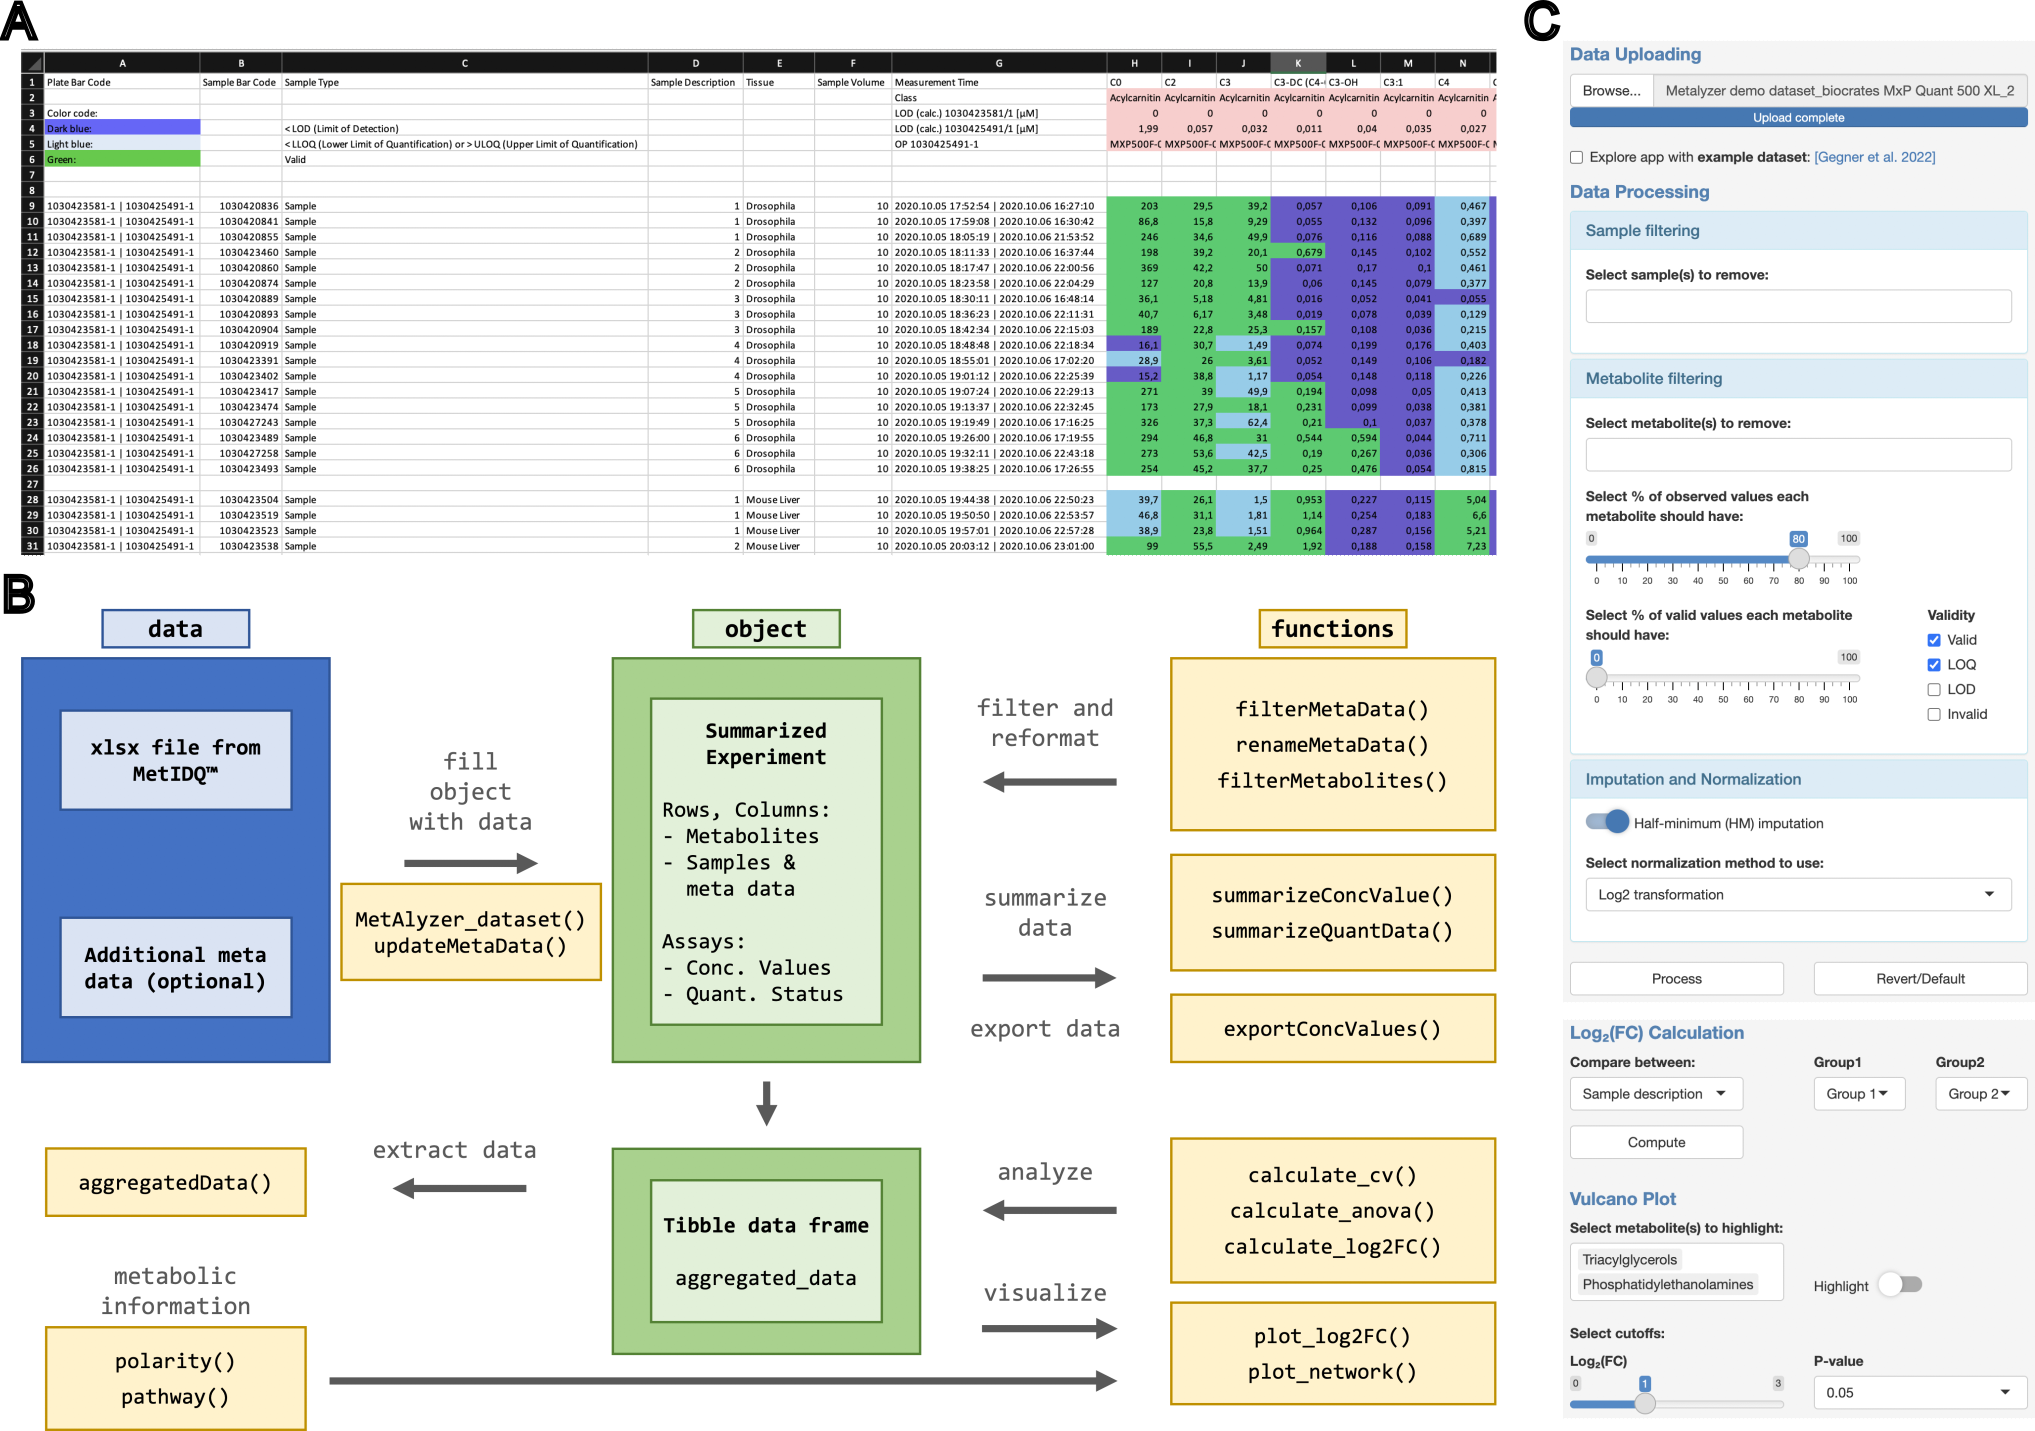
\includegraphics[scale=1.1]{figure1.png}
    \caption{\textbf{Overall features of MetAlyzer} | \textbf{(A)} An example Excel spreadsheet exported from Biocrates' WebIDQ contains metabolite concentrations along with sample and metabolite metadata and color-coded quantification statuses. \textbf{(B)} The workflow of MetAlyzer begins by converting a Biocrates-exported spreadsheet into a \textit{SummarizedExperiment} object to which sample and metabolite filtering, data imputation and transformation, and various analyses including descriptive statistics, fold changes, and ANOVA are applied. The statistical results can be visualized using volcano and scatter plots and network diagrams. \textbf{(C)} The Shiny-based graphical interface of MetAlyzer provides point-and-click access to the full analysis workflow.}
    \label{fig:overallFeatures}
\end{figure}

\subsection*{\normalsize Usage scenario}
We demonstrate the utility of MetAlyzer through its Shiny app using a demo dataset generated with the MxP® Quant 500 XL kit, provided by our collaborators at Biocrates. The raw dataset, exported directly from the WebIDQ software, was uploaded onto the app and initially assessed in terms of its data distribution, missingness patterns, and quantification status composition to guide the selection of appropriate preprocessing steps. Given that the overall quantification appeared stable and no systematic distributional drift was evident (Fig.~\ref{fig:usageScenario}A,B), we applied metabolite filtering based on the 80\% rule\cite{Wei2018} to enhance statistical robustness, followed by $\log_2$ transformation to stabilize variance across the dataset. We then performed statistical comparisons between the samples from Group 1 and Group 2, identifying differentially abundant metabolites, particularly within the triacylglycerol (TAG) and glycerophospholipid (GPL) classes (Fig.~\ref{fig:usageScenario}C,D). The volcano and scatter plots indicated higher enrichment of TAGs in Group 1, while GPLs were more enriched in Group 2. Finally, the network diagram highlighted potential perturbations in polyamine, indole/tryptophan, and lysine metabolic pathways (Fig.~\ref{fig:usageScenario}E).

\begin{figure}[b!]
    \centering
    \caption{\textbf{Utility of MetAlyzer demonstrated using demo dataset consisting of two biologically different sample groups} | \textbf{(A)} The boxplot of the unprocessed data, colored by the two sample groups, showed substantial variance across the dataset but no evident systematic distributional drift. The central line of each box is the median; the box hinges span the 25\textsuperscript{th} to 75\textsuperscript{th} percentiles, while the whiskers extend up to 1.5 times the interquartile range beyond the hinges. Outliers are displayed as individual points outside the whiskers. \textbf{(B)} The barplot illustrated missingness patterns across samples in the unprocessed data, suggesting that the overall quantification was stable. \textbf{(C)} The volcano plot identified differentially abundant metabolites in the comparison of Group 1 and Group 2 samples, particularly within the triacylglycerol (TAG; brown) and phosphatidylethanolamine (PE; yellow) classes. TAGs were more enriched in Group 1 and PEs in Group 2. The thresholds for $\log_2$ fold change (FC) and p-value were set at 1 and 0.05, respectively. Colors assigned to points denote metabolic classes. \textbf{(D)} The scatter plot complements the volcano plot, illustrating differentially abundant TAGs and GPLs (e.g., PAs, PCs, PEs). Points are colored by q-values; background rectangles indicate metabolic classes. \textbf{(E)} The network diagram revealed potential disruptions in polyamine, indole/tryptophan, and lysine metabolic pathways. Colors of nodes and edges denote $\log_2$ FCs of metabolites and indicate their involvement in specific pathways.}
    \label{fig:usageScenario}
\end{figure}

\begin{figure}[t!]
    \centering
    \hspace*{-5mm}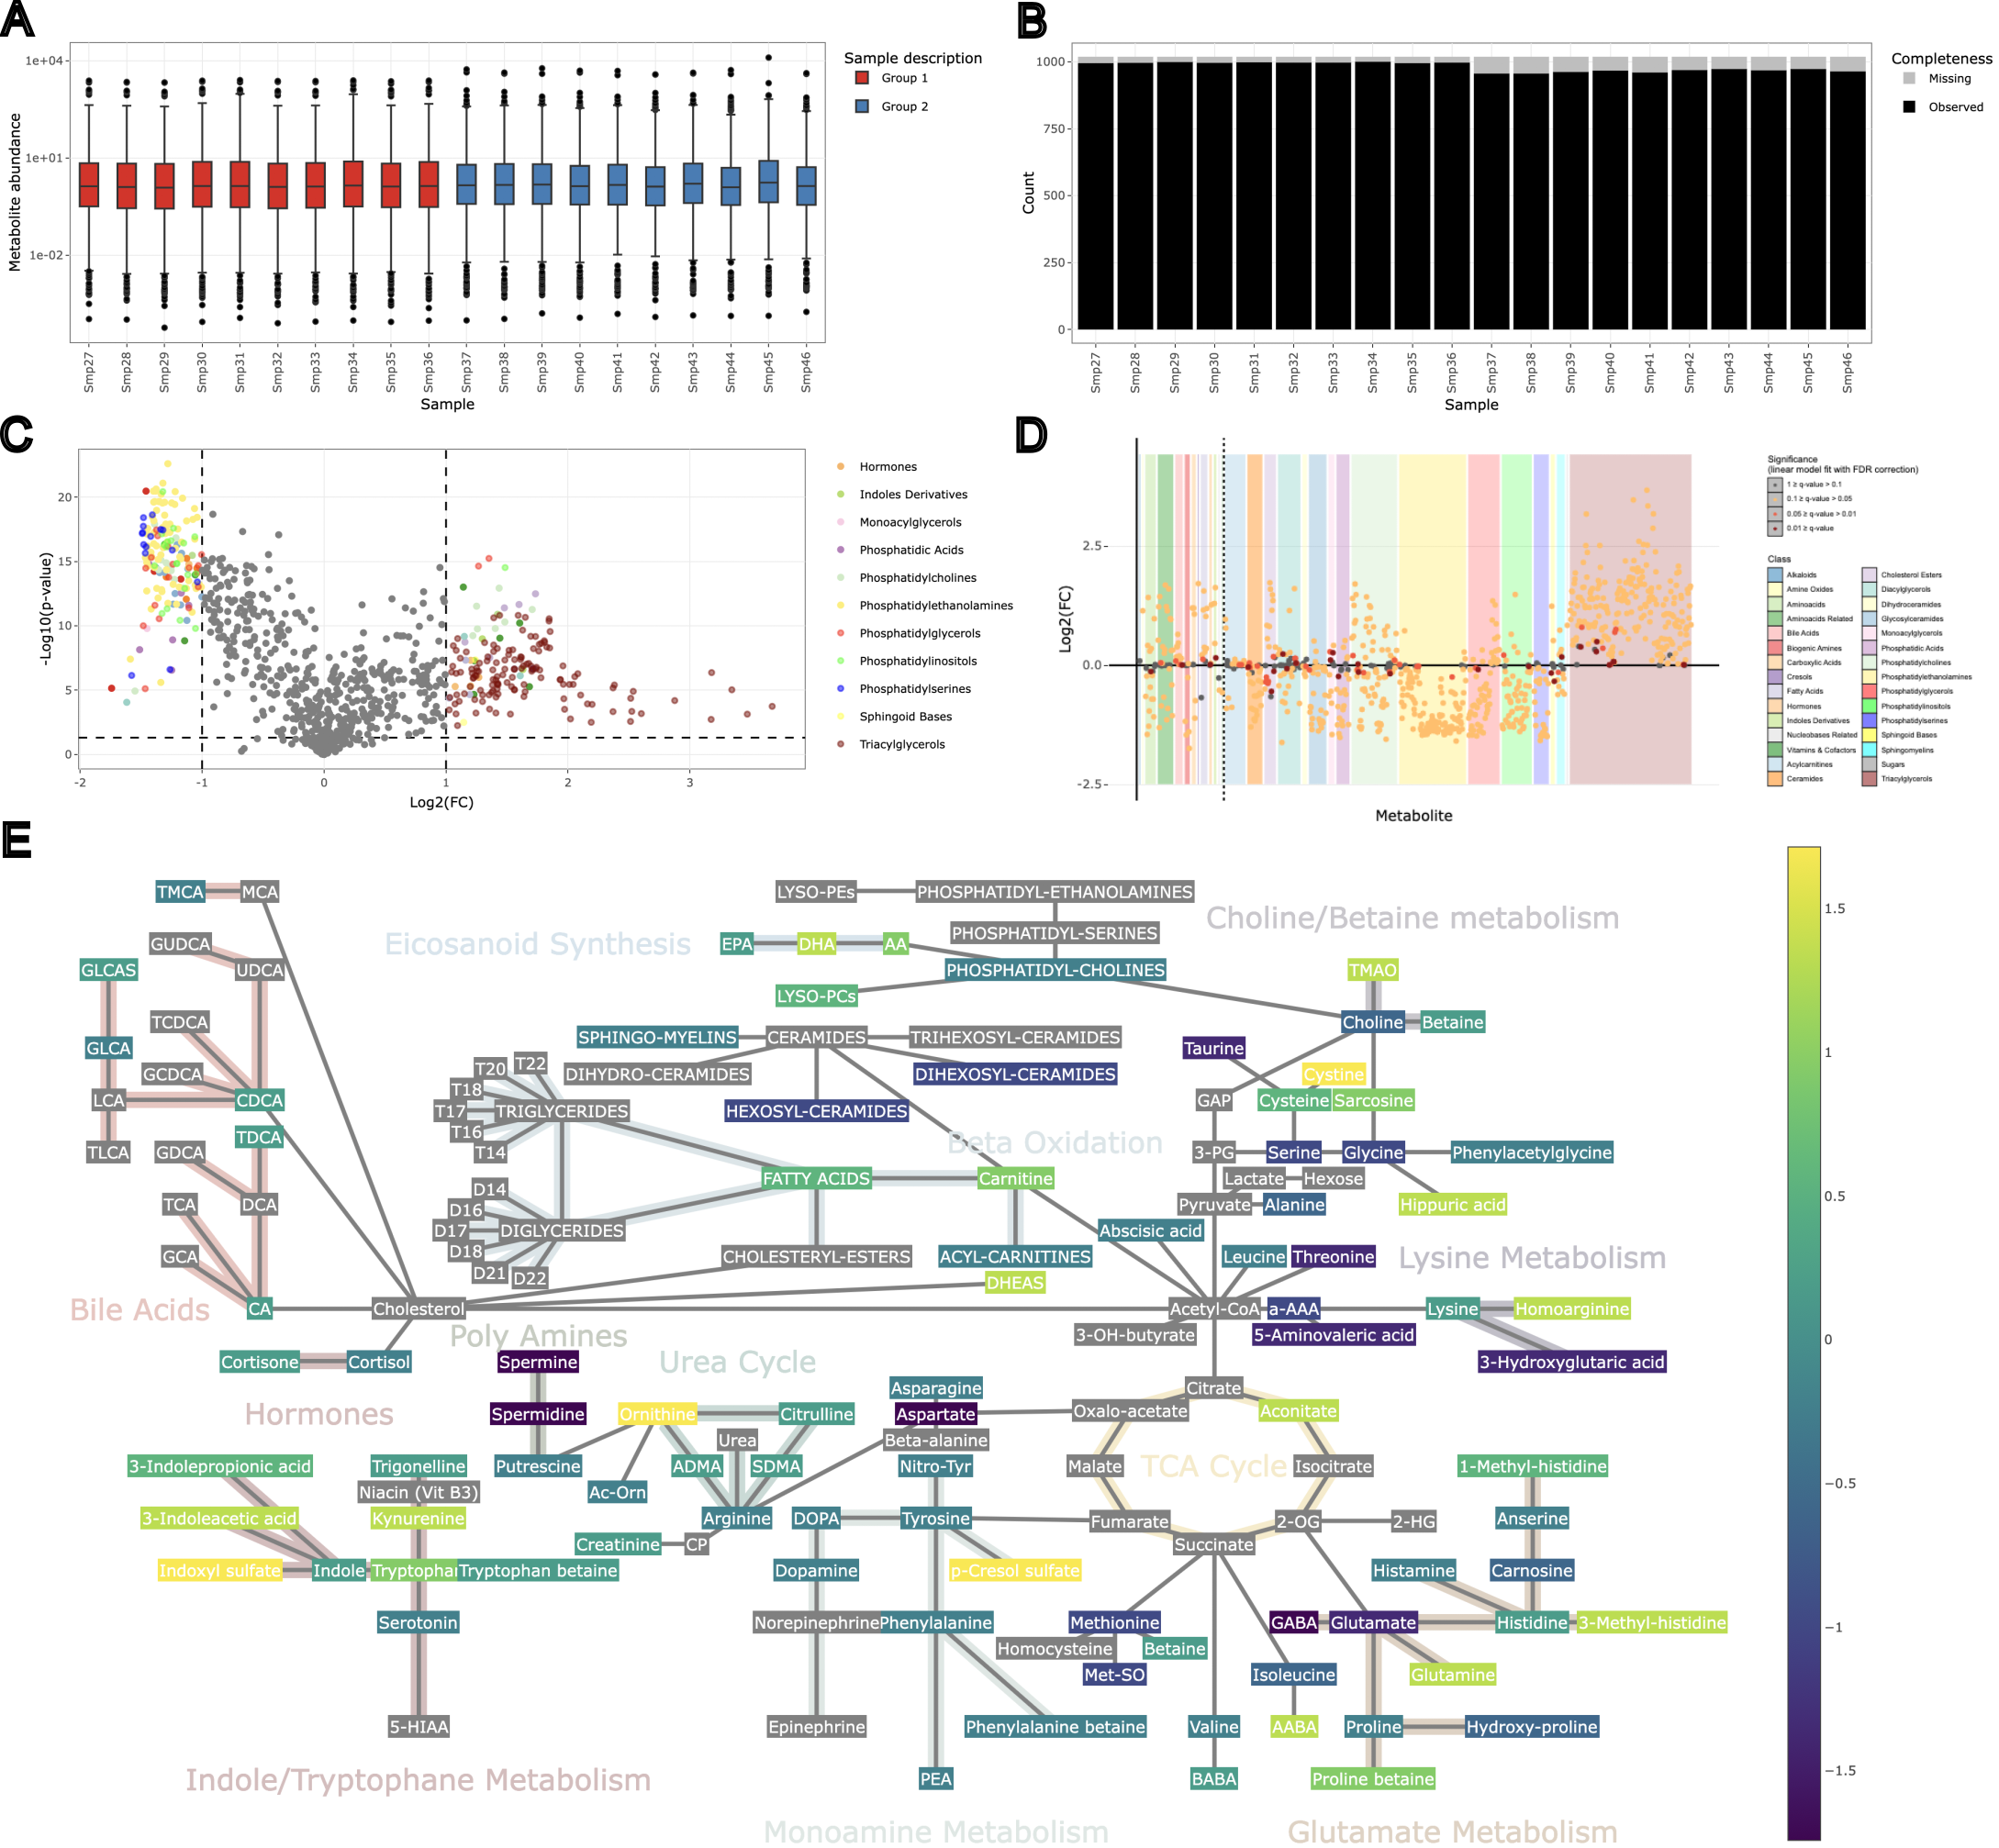
\includegraphics[scale=1.1]{figure2_2.png}
\end{figure}

% \section*{\large Implementation}
% After kit raw MS data is processed by biocrates' \textbf{MetIDQ} software, one can upload the output Excel spreadsheet onto MetAlyzer's shiny app, of which the standard implementation is described as follows:
% \newline
% \indent (1) Data upload. Note that uploaded data should be an Excel spreadsheet (.xlsx format) exported from biocrates' \textbf{MetIDQ} software, where the column "Sample Type" and the row "Class" must be present and fixed as the original, since these two cells are used as anchors to convert a spreadsheet into a \textit{SummarizedExperiment} object.
% \newline
% \indent (2) Data overview and preprocessing. The uploaded data can be first viewed from different angles to determine whether further preprocessing is needed. Our app provides a boxplot displaying the distributions of metabolite concentrations across samples, a barplot illustrating the proportions of missing values and quantification statuses of metabolites in samples, and a table showing sample metadata. For preprocessing, options for sample and metabolite filtering, imputation, and normalization are available. Filtering can be performed on individual or grouped samples and metabolites, or by setting cutoffs for metabolite missingness and invalid quantification status levels. Imputation is done using the half-minimum approach, while normalization can be achieved through either median normalization or total ion count normalization. The plots update once the data is processed, providing an immediate overview of the effect of each operation. Additionally, all processing parameters and resulting plots from each operation are stored in the history table, allowing for comparisons between different trials and ensuring traceability.
% \newline
% \indent (3) Data analysis. Statistical analysis can then be performed to identify differential metabolites between two sample groups, from which log2 fold changes and p-values are calculated. To visualize differential analysis results, a volcano plot, scatter plot, and network plot are provided. Specifically, the scatter plot illustrates the relationships between log2 fold changes and metabolic classes, helping to reveal whether any class is differentially abundant. The network plot displays the predefined canonical metabolic pathways, with nodes annotated by calculated statistics to highlight key metabolites and their interconnections. All plots can be downloaded to a local computer.

% Last, our app allows users to download alternative metabolite identifiers, such as HMDB IDs, corresponding to metabolites named by biocrates using their nomenclature \textit{(biocrates-named compounds)}. These identifiers can then be used for further analysis, for instance, pathway analysis through MetaboAnalyst\cite{Pang2024}.

\section*{\large Discussion}
MetAlyzer is an R package designed for the efficient processing and analysis of targeted metabolomics datasets exported from the Biocrates platform. Its strengths lie in a streamlined, dual-mode workflow that integrates both a code-based interface and an interactive Shiny app. The workflow begins by converting a complex Biocrates-exported Excel spreadsheet into a flexible \textit{SummarizedExperiment} object\cite{Morgan2022}, which serves as the central data structure within MetAlyzer and can also be widely used in external environments (e.g., Bioconductor\cite{Huber2015}), enhancing interoperability and customizability. The workflow is minimal yet functionally complete, encompassing sample and metabolite filtering, data imputation and transformation, statistical analysis, and result visualization, which supports rapid quality control and downstream analysis. Although Biocrates' WebIDQ software has its own data cleaning (modified 80\% rule\cite{Wei2018}) and imputation (k-nearest neighbors) methods, MetAlyzer provides complementary options, such as filtering by metabolite quantification statuses and imputation using the half-minimum approach.

To improve accessibility and efficiency, the Shiny-based interface enables full workflow execution without requiring users to code, particularly valuable for wet-lab or medical researchers with limited to no programming experience. Unlike existing web-based tools\cite{Pang2024,Galaxy2024,MWB}, MetAlyzer directly accepts raw Biocrates-exported spreadsheets and includes only essential steps, which reduces complexity while supporting flexible data exploration and hypothesis generation. Recognizing that users may require more advanced analyses, we plan to extend MetAlyzer's functionality by exporting compatible data formats (e.g., concentration matrices) for use in other tools (e.g., MetaboAnalyst for enrichment analysis\cite{Xia2010}).

Altogether, MetAlyzer offers an accessible and efficient solution for the reproducible analysis of targeted metabolomics data generated with the Biocrates platform, which balances usability and flexibility through a dual interface that supports both routine tasks and exploratory research across varying levels of user expertise.

\section*{\large Data availability}
\vspace{-4mm}
The demo dataset used in this study is available in the GitHub repository \textit{LiaoQianWu/RShiny\_Biocrates\_DA} at \url{https://github.com/LiaoQianWu/RShiny_Biocrates_DA}.

\section*{\large Code availability}
\vspace{-4mm}
The MetAlyzer package is publicly available in the GitHub repository \textit{nilsmechtel/MetAlyzer} at \url{https://github.com/nilsmechtel/MetAlyzer} and released under the GPL-3.0 license. The code for the Shiny-based MetAlyzer application is available in the GitHub repository \textit{LiaoQianWu/RShiny\_Biocrates\_DA} at \url{https://github.com/LiaoQianWu/RShiny_Biocrates_DA}.

\section*{\large Additional information}
\vspace{-4mm}
Vignettes for both the code-based and Shiny-based versions of MetAlyzer are available in the GitHub repositories \href{https://github.com/nilsmechtel/MetAlyzer}{\textit{nilsmechtel/MetAlyzer}} and \href{https://github.com/LiaoQianWu/RShiny_Biocrates_DA}{\textit{LiaoQianWu/RShiny\_Biocrates\_DA}}, respectively.

\setstretch{1}
\bibliographystyle{unsrt}
% \nocite{*}
\footnotesize
\bibliography{references}

\end{document}